\documentclass[10pt,conference]{IEEEtran}
\IEEEoverridecommandlockouts

\usepackage[utf8]{inputenc}
\usepackage[T1]{fontenc}
\usepackage[brazilian]{babel}
\usepackage{cite}
\usepackage{amsmath,amssymb,amsfonts}
\usepackage{graphicx}
\usepackage{textcomp}
\usepackage{xcolor}
\usepackage{booktabs}
\usepackage{url}
\usepackage{balance}
\usepackage{enumitem}

\begin{document}

\title{Que Skills de Teste as Agent Skills Ensinam?\\
Um Perfil Preliminar via Practical Test Pyramid no GitSkills}

\author{\IEEEauthorblockN{Pamella Soares}
\IEEEauthorblockA{Universidade Estadual do Ceará (UECE)\\
Fortaleza, Brasil\\
pamella.soares@aluno.uece.br}
}

\maketitle

\begin{abstract}
Agent skills (\texttt{SKILL.md}) instruem coding agents em linguagem natural, sem compilador que valide a orientação de teste.
Neste \emph{short paper} do MSR~2027 Mining Challenge, perguntamos quais \textbf{skills de teste} são evidenciadas em skills do domínio blockchain no dataset GitSkills.
Operacionalizamos a \emph{Practical Test Pyramid} (Vocke/Fowler) como glossário de \textbf{níveis de teste} e de skills relacionadas (Unitário, Integração, Contrato, UI, E2E, Aceitação, Exploratório, Automação).
A partir de 89.649 skills com vocabulário blockchain, filtramos 17.847 com orientação lexical a teste: Unitário (30,0\%) e Integração (23,6\%) dominam; E2E (14,3\%) e Aceitação (2,8\%) são menos frequentes; sinais Web3 como fuzz/invariant (9,9\%) e fork (2,8\%) aparecem aquém de coverage/regression.
Discutimos os \textbf{impactos} desses desequilíbrios para o desenvolvimento de sistemas baseados em blockchain (falsos verdes, superfície DeFi, pontes, carteiras e governança de agentes).
Um piloto LLM (checklist com evidência verbatim) e uma amostra cega estratificada ($n{=}32$) sustentam o protocolo.
Não medimos proficiência---apenas \emph{skill evidenciada} no texto.
\end{abstract}

\begin{IEEEkeywords}
Mining Software Repositories, GitSkills, agent skills, test pyramid, blockchain, testing skills
\end{IEEEkeywords}

\section{Introdução}

Agent skills são pastas com um \texttt{SKILL.md} que orienta um agente de IA sobre como executar tarefas~\cite{gitskills2027}.
Diferente de código, o conteúdo é predominantemente linguagem natural: não há type checker que diga se a orientação de teste é completa ou adequada ao domínio.
Em sistemas baseados em blockchain e DApps, falhas de verificação têm custo alto---fundos imobilizados, exploits, estado on-chain difícil de reverter e risco reputacional para protocolos.

A pilha prática de verificação Web3 não se reduz a ``rodar unit tests'': inclui integração entre aplicação, contrato e rede; testes de ponta a ponta; propriedades/invariantes; fuzzing; forks de mainnet; e critérios de oráculo (reverts, eventos, saldo, autorização).
Quando um coding agent é guiado por skills incompletas, o risco não é apenas acadêmico: o agente pode gerar ou modificar contratos e scripts de deploy com uma suíte que parece suficiente e ainda assim omite níveis críticos.

O MSR~2027 Mining Challenge disponibiliza o GitSkills~\cite{gitskills2027} e incentiva taxonomias de propósito e métricas para instruções em linguagem natural.
Este artigo responde, de forma preliminar:

\begin{itemize}[leftmargin=*,itemsep=1pt]
\item \textbf{RQ1 (quantitativa):} Com que frequência skills blockchain mencionam cada \textbf{nível de teste} da pirâmide prática (e sinais correlatos Web3)?
\item \textbf{RQ2 (qualitativa/piloto):} Quais \emph{testing skills} o texto evidencia quando anotado via checklist da Practical Test Pyramid?
\item \textbf{Impacto:} O que esses padrões implicam para quem desenvolve, audita ou opera sistemas blockchain com auxílio de agentes?
\end{itemize}

\paragraph{Escopo.}
Não propomos taxonomia ISTQB/ISO completa; adotamos o vocabulário operacional de Vocke/Fowler~\cite{vocke2018pyramid}, que alerta para ambiguidade de nomes de níveis.
Classificamos \emph{skill evidenced / skill instructed}, não proficiência do autor.
Não afirmamos causalidade entre skill e defeito em produção; discutimos \emph{riscos plausíveis} à luz da literatura prática de verificação on-chain.

\section{Referência: Practical Test Pyramid}

A pirâmide clássica (Cohn) agrupa testes por granularidade: muitos testes de baixo nível, poucos de alto nível, buscando feedback rápido e custo controlado.
Vocke~\cite{vocke2018pyramid} discute Unit, Integration, Contract, UI, End-to-End e Acceptance, além de Exploratory e automação/CI como preocupações transversais.
Acceptance é \textbf{ortogonal} à pirâmide (não forçamos ``aceitação = topo'').
Para mineração com LLM, isso motiva um checklist curto (Q1--Q8) em vez de uma taxonomia de técnicas/tipos.

No domínio blockchain, os mesmos níveis ganham significados concretos: unitário sobre funções de contrato ou bibliotecas; integração entre serviços off-chain e contratos; contrato no sentido de interfaces consumidor--provedor (p.ex., oráculos, bridges); UI/API de carteiras e front-ends; E2E atravessando usuário$\rightarrow$API$\rightarrow$contrato$\rightarrow$cadeia; aceitação alinhada a requisitos de negócio/protocolo.

\section{Metodologia}

\subsection{Visão geral (pipeline)}
\begin{enumerate}[leftmargin=*,itemsep=1pt]
\item Partir do snapshot GitSkills (coleta jul/2026; linhagem \texttt{agent\_skills\_mandatory\_only}).
\item Restringir a skills com $\geq$1 termo blockchain (\emph{mandatory terms}).
\item Filtrar lexicalmente orientação a teste / níveis de teste (pool candidato).
\item Agregar prevalência por nível (RQ1), exclusiveidade e coocorrência.
\item Amostrar piloto e aplicar checklist Pyramid via LLM (RQ2).
\item Preparar amostra cega estratificada para validação humana.
\item Interpretar resultados sob a ótica de impacto em desenvolvimento blockchain.
\end{enumerate}

\subsection{Dados}
\begin{itemize}[leftmargin=*,itemsep=1pt]
\item \textbf{Dataset:} GitSkills~\cite{gitskills2027}, versão alinhada ao desafio (jul/2026).
\item \textbf{Base analítica:} \texttt{agent\_skills\_mandatory\_only.db} --- 89.649 skills distintas (\texttt{dedup\_primary=1}) com $\geq$1 termo blockchain.
\item \textbf{Unidade:} um artefato \texttt{SKILL.md} (\texttt{name}, \texttt{description}, \texttt{content}).
\item Toda a trilha parte de \texttt{mandatory\_only} (não da base \texttt{blockchain\_filtered} alternativa).
\end{itemize}

\subsection{Filtro lexical por nível de teste (RQ1)}
\begin{itemize}[leftmargin=*,itemsep=1pt]
\item Vocabulário em frases compostas (evita o termo isolado ``test''); busca case-insensitive em conteúdo+nome+descrição.
\item Níveis nucleares: \emph{unitário}, \emph{integração}, \emph{ponta a ponta (E2E)}, \emph{aceitação}.
\item Sinais adicionais (não substituem o nível): coverage, regression, fork, fuzz/property, mutation, gas/performance, etc.
\item Entrada no pool: $\geq$1 termo em qualquer grupo $\Rightarrow$ \textbf{17.847} skills ($\approx$19,9\% da base blockchain lexical).
\item Multi-rótulo lexical permitido; reportamos prevalência ``qualquer menção'' e contagens exclusivas.
\item Artefatos: listas de termos, pool JSON, scripts de filtragem e plots.
\end{itemize}

\subsection{Checklist Pyramid e piloto LLM (RQ2)}
\begin{itemize}[leftmargin=*,itemsep=1pt]
\item Instrumento Q1--Q8: Unitário, Integração, Contrato, UI, E2E, Aceitação, Exploratório, Automação.
\item Respostas: \texttt{YES}/\texttt{NO}/\texttt{UNCERTAIN}; todo \texttt{YES} exige quote verbatim.
\item A LLM responde o checklist; regras em código derivam \texttt{skills\_evidenced} só com quote validável.
\item Princípios: multi-rótulo com evidência independente; exploratory só com menção explícita; não avaliar qualidade.
\item Piloto: 6 skills (3 exemplos de pirâmide + 3 do pool); 5 classificadas como orientação a teste.
\end{itemize}

\subsection{Validação humana (em andamento)}
\begin{itemize}[leftmargin=*,itemsep=1pt]
\item Amostra cega: \textbf{8} skills por nível lexical exclusivo $\times$ 4 níveis $=$ \textbf{$n{=}32$} (seed 20270402).
\item Revisores não veem o estrato lexical; protocolo em \texttt{PROTOCOL\_MANUAL\_REVIEW.md}.
\item $\kappa$/$\alpha$ após dupla anotação entram na versão estendida; aqui reportamos o desenho.
\end{itemize}

\section{Resultados}

\subsection{RQ1 --- Prevalência por nível de teste}
No pool ($n{=}17.847$), a prevalência lexical (não exclusiva) é resumida na Tabela~\ref{tab:prev} e nas Figuras~\ref{fig:prev}--\ref{fig:pyr}.

\begin{table}[t]
\centering
\caption{Prevalência lexical no pool de orientação a teste.}
\label{tab:prev}
\setlength{\tabcolsep}{3.5pt}
\begin{tabular}{@{}lrrr@{}}
\toprule
Nível / sinal & Skills & \% pool & Exclusivo \\
\midrule
Unitário & 5.348 & 30,0 & 2.240 \\
Integração & 4.215 & 23,6 & 1.302 \\
E2E & 2.552 & 14,3 & 751 \\
Aceitação & 496 & 2,8 & 326 \\
\midrule
Coverage & 5.344 & 29,9 & --- \\
Regression & 4.748 & 26,6 & --- \\
Fuzz / property & 1.772 & 9,9 & --- \\
Fork & 497 & 2,8 & --- \\
\bottomrule
\end{tabular}
\end{table}

Além disso: 3.295 skills (18,5\%) combinam $\geq$2 níveis nucleares (coocorrência mais frequente: unitário+integração, 2.739); 9.933 skills (55,7\%) entram no pool por sinais de teste \emph{sem} mencionar os quatro níveis nucleares---muitas via coverage/regression ou outros tipos.
Isso indica um corpus em que ``falar de teste'' frequentemente não especifica \emph{qual} nível da pirâmide praticar.

\begin{figure}[t]
\centering
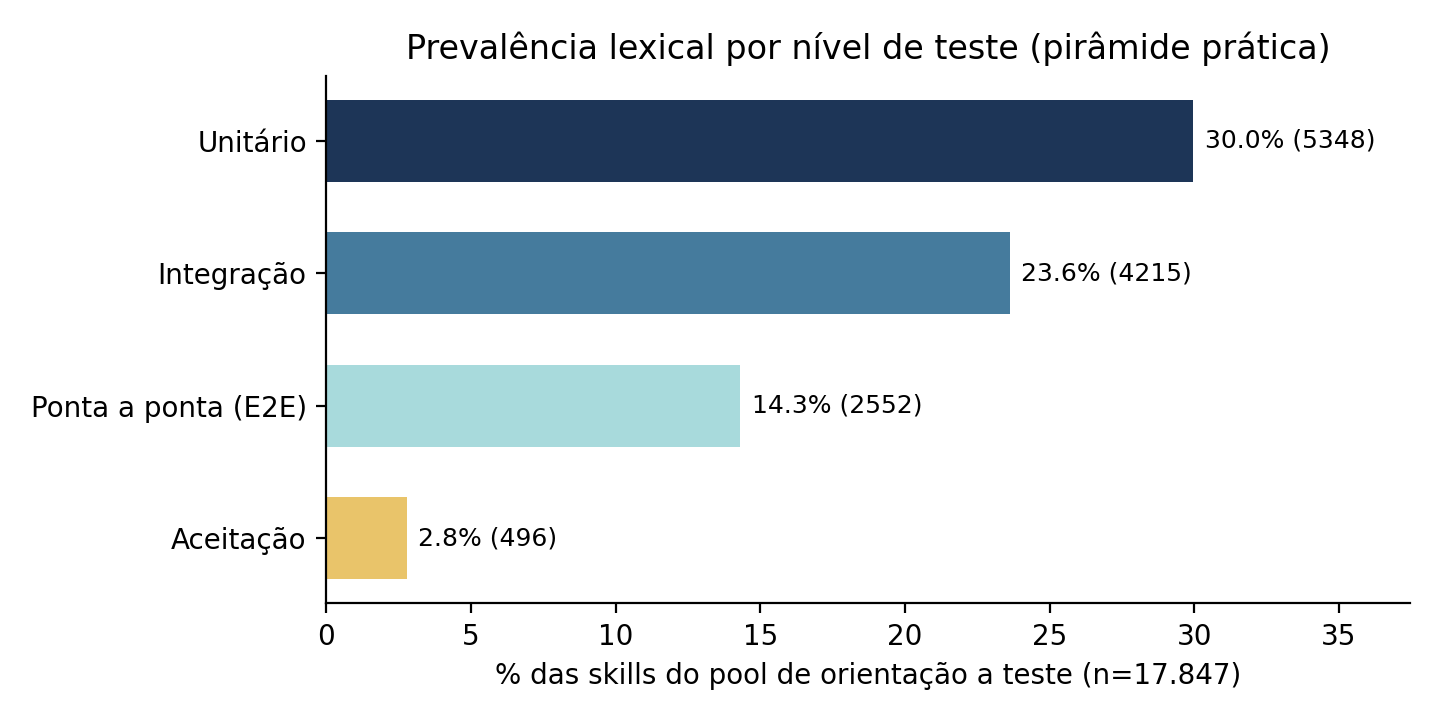
\includegraphics[width=\columnwidth]{figures/fig_nivel_prevalence.png}
\caption{Prevalência lexical por nível de teste ($n{=}17.847$).}
\label{fig:prev}
\end{figure}

\begin{figure}[t]
\centering
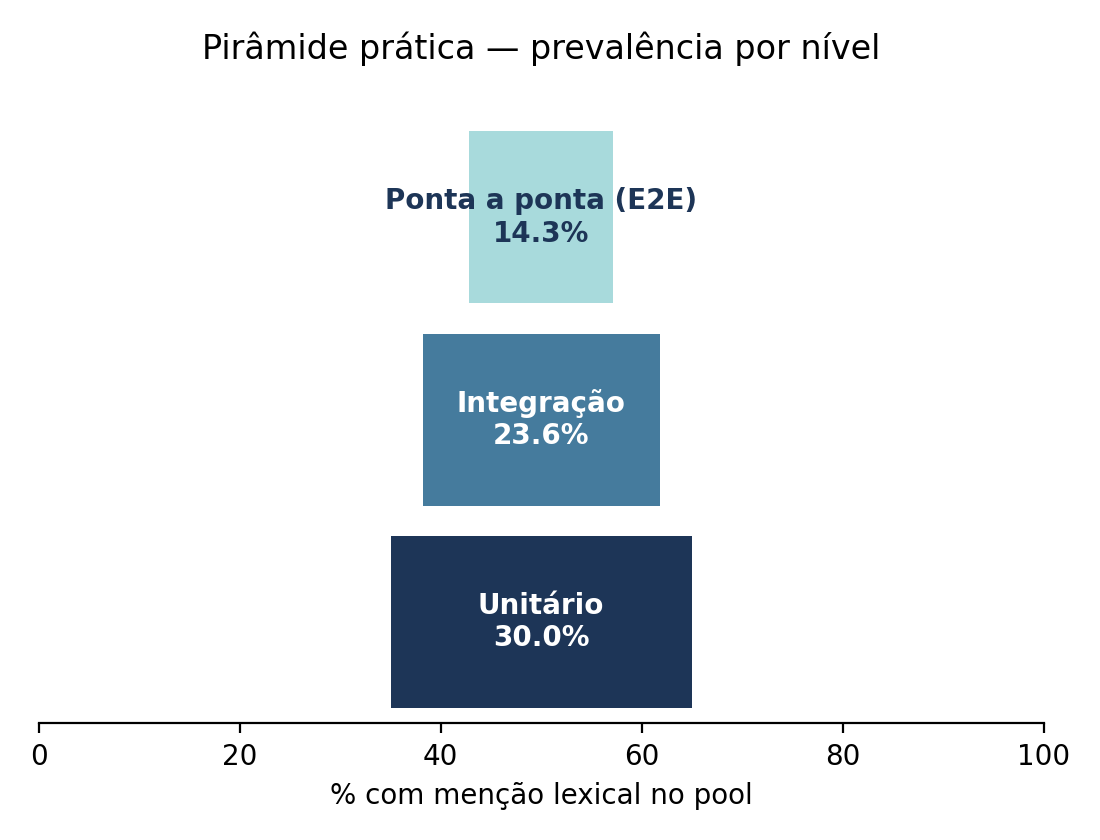
\includegraphics[width=0.92\columnwidth]{figures/fig_pyramid_niveis.png}
\caption{Pirâmide prática: Unitário, Integração e E2E (\% do pool).}
\label{fig:pyr}
\end{figure}

\subsection{RQ2 --- Testing Skill Profile (piloto)}
Nas 5 skills com orientação a teste no piloto LLM, Automação apareceu em 4/5; Unitário, Integração e Contrato em 3/5; UI e E2E em 2/5; Aceitação e Exploratório em 0/5 (Figura~\ref{fig:prof}).
Exemplos qualitativos: uma skill de desenvolvimento Solidity enfatizou unitário+cheatcodes/asserções; uma de pentest de DApps evidenciou integração backend--blockchain, UI/XSS em carteiras e E2E de fluxos; skills com fuzz/fork no texto lexical tenderam a evidenciar automação e técnicas de propriedade---mas Aceitação e Exploratório permaneceram ausentes.
Quotes não verbatim foram descartadas automaticamente.

\begin{figure}[t]
\centering
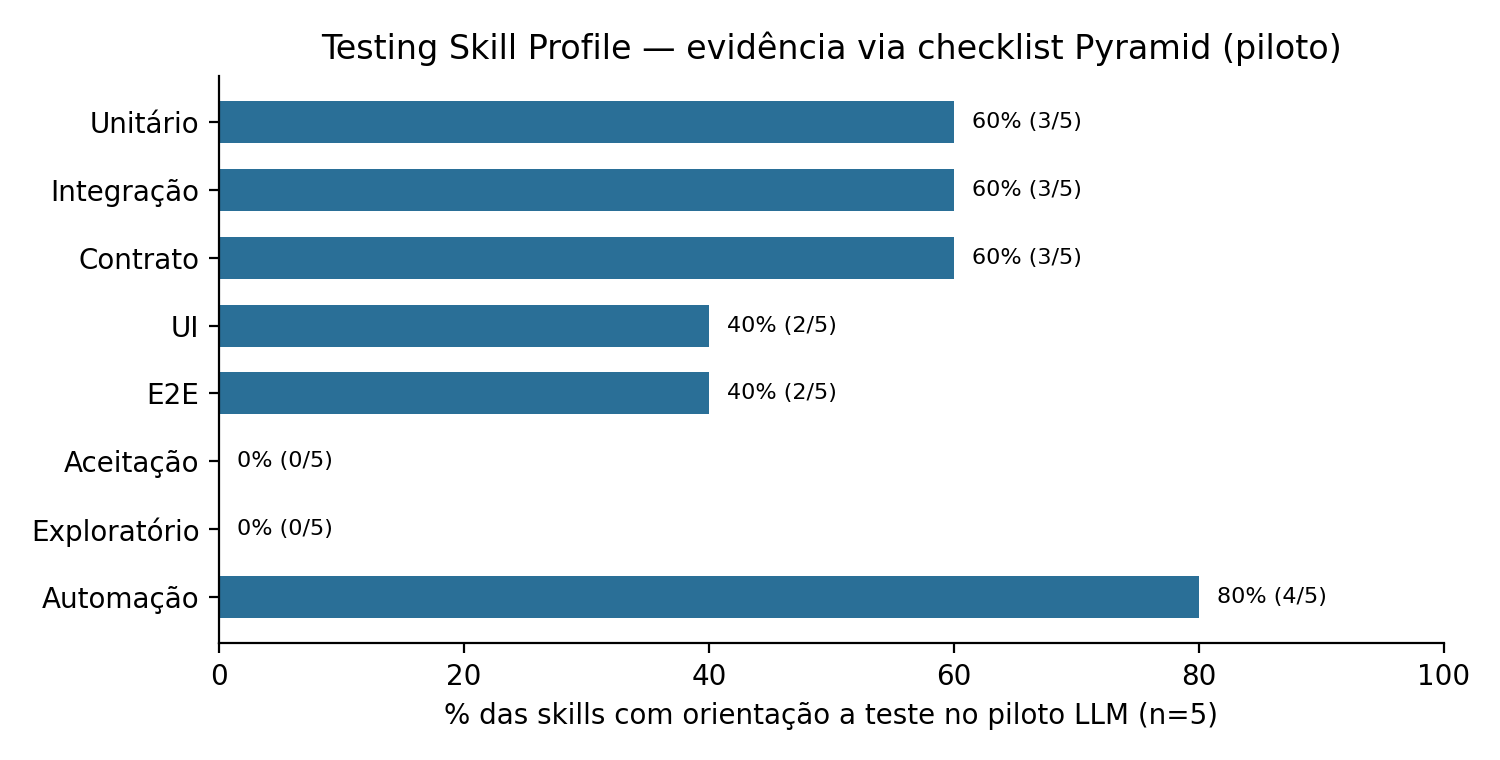
\includegraphics[width=\columnwidth]{figures/fig_skill_profile_piloto.png}
\caption{Cobertura de skills evidenciadas no piloto LLM.}
\label{fig:prof}
\end{figure}

\section{Impactos para o desenvolvimento de sistemas blockchain}

Os números não medem defeitos em produção; medem o que as \emph{instruções} disponíveis aos agentes enfatizam.
Em um ecossistema onde agents passam a escrever, refatorar e ``validar'' contratos, esse viés de instrução torna-se parte do risco de engenharia.
Organizamos os impactos por nível omitido ou sub-representado.

\subsection{Unitário frequente, porém insuficiente sozinho}
Unitário é o nível mais citado (30,0\%).
Para bibliotecas Solidity/Vyper e lógica pura, isso é positivo: feedback rápido, asserts de revert/evento, isolamento.
O impacto negativo aparece quando a skill (e, por extensão, o agente) trata unitário como \emph{definição} de ``bem testado''.
Em DeFi, muitos exploits exploram interações, ordem de mensagens, oráculos e estados compostos---cenários que unitários com mocks agressivos podem mascarar.
\textbf{Impacto prático:} times que confiam em agents guiados por skills unit-cêntricas podem acelerar entrega com cobertura aparente alta e ainda assim deixar aberta a superfície de integração.

\subsection{Integração presente, mas assimétrica}
Integração (23,6\%) é o segundo nível nuclear.
Isso é encorajador para pontes app$\leftrightarrow$contrato e sync off-chain/on-chain.
Contudo, coocorrência forte com unitário (2.739 skills) sugere que ``integração'' muitas vezes aparece no mesmo pacote retórico genérico, sem garantir profundidade (p.ex., testes com nó real, anvil/hardhat network, ou dependências externas verdadeiras).
\textbf{Impacto:} em carteiras, indexadores e backends de DApp, falhas de integração geram transações mal formadas, nonces inconsistentes e estados divergentes---exatamente o tipo de defeito que usuários finais percebem como ``a blockchain falhou'', embora a falha seja de composição de sistemas.

\subsection{E2E relativamente raro (14,3\%)}
E2E exercita o fluxo completo via interface externa.
Em blockchain, isso frequentemente significa: carteira$\rightarrow$front$\rightarrow$RPC$\rightarrow$contrato$\rightarrow$eventos/indexação.
A menor prevalência implica que agents podem ser pouco instruídos a validar jornadas reais (mint, swap, stake, bridge) sob condições de rede.
\textbf{Impacto:} regressões de UX e de caminho feliz/infeliz em produção; custo operacional de suporte; em pior caso, usuários assinando fluxos parcialmente quebrados.
Skills E2E genéricas (p.ex., Playwright Web2) sem oráculos on-chain ainda podem dar falso conforto.

\subsection{Aceitação quase ausente (2,8\%)}
Aceitação---cenários de negócio/stakeholder---é rara no léxico das skills.
Protocolos blockchain codificam regras econômicas e de governança: limites de mint, papéis, upgrades, pausas, taxa.
Sem aceitação explícita, o agente pode ``passar nos testes'' sem verificar se a \emph{feature} atende à especificação de negócio ou ao whitepaper operacional.
\textbf{Impacto:} desalinhamento entre requisito econômico e implementação; auditorias tardias descobrem que o comportamento testado não é o comportamento desejado pelo protocolo.

\subsection{Fuzz/invariant e fork sub-representados}
Fuzz/property (9,9\%) e fork (2,8\%) ficam bem abaixo de coverage (29,9\%) e regression (26,6\%).
Na prática BOSE, fuzz/invariant e forks de mainnet são ferramentas centrais para estados raros, propriedades DeFi e reproducão de condições reais de liquidez/slots.
Coverage/regression, embora úteis, não substituem busca adversária de estado.
\textbf{Impacto:} agents otimizando para ``coverage report verde'' em vez de propriedades quebráveis; menor chance de detectar edge cases que auditores e hunters buscam; risco particularmente alto em upgrades e em composabilidade DeFi.

\subsection{Automação sem pirâmide completa}
No piloto, Automação foi a skill mais frequente entre as evidenciadas.
Automatizar uma suíte enviesada para a base da pirâmide \emph{acelera} o viés: CI passa rápido, o agente recebe reforço positivo, e níveis altos/raros continuam omitidos.
\textbf{Impacto:} pipelines que institucionalizam o falso verde; governança frágil de ``definition of done'' para PRs gerados por IA.

\subsection{Síntese para papéis do ecossistema}
\begin{itemize}[leftmargin=*,itemsep=2pt]
\item \textbf{Times de protocolo/DeFi:} tratar skills unit-cêntricas como incompletas por padrão; exigir invariantes, fuzz e cenários de integração/composição no Definition of Done do agente.
\item \textbf{Carteiras e front-ends:} priorizar skills com UI/API + E2E que incluam assinatura, cadeia e falhas de RPC---não apenas testes de componente React.
\item \textbf{Bridges e oráculos:} enfatizar contract/integration testing e forks; o custo de falha de interface é sistêmico.
\item \textbf{Auditores e securidade:} usar o gap (aceitação/E2E/fuzz/fork) como checklist de revisão de PRs assistidos por agentes.
\item \textbf{Autores de skills / marketplaces:} publicar skills com perfil de pirâmide explícito (quais níveis instrui) para reduzir overtrust.
\item \textbf{Pesquisadores MSR:} o \emph{Testing Skill Profile} oferece métrica de qualidade de instrução alinhada ao challenge (propósito + evidência).
\end{itemize}

\section{Ameaças à validade}

\begin{itemize}[leftmargin=*,itemsep=1pt]
\item \textbf{Construto:} menção lexical $\neq$ orientação acionável; mitigamos parcialmente com checklist+quote na RQ2.
\item \textbf{Interna:} overclassification LLM; quotes inválidas descartadas; piloto pequeno ($n{=}6$).
\item \textbf{Externa:} base \texttt{mandatory\_only} tem alto recall (ruído de termos ambíguos); skills espelham templates, não necessariamente prática de protocolos top-tier.
\item \textbf{Conclusão:} impactos são \emph{riscos plausíveis}, não efeitos medidos em mainnet.
\item Ambiguidade de nomes de níveis (reconhecida por Vocke/Fowler); amostra humana ainda sem $\kappa$ publicado.
\end{itemize}

\section{Implicações Éticas}

Analisamos artefatos públicos do GitSkills.
Não reidentificamos autores além dos metadados do dataset.
A amostra cega reduz viés de confirmação dos revisores.
Não executamos skills nem comandos nelas prescritos.
Discussões de impacto não devem ser lidas como acusação a repositórios específicos.

\section{Conclusão}

Nas agent skills blockchain do GitSkills, a orientação a teste concentra-se nos níveis unitário e de integração e em proxies como coverage/regression; E2E, aceitação, fuzz/property e fork são comparativamente raros.
Para o desenvolvimento de sistemas blockchain, isso significa um risco estrutural de \emph{overtrust} em agentes: acelerar implementação com feedback automatizado na base da pirâmide, enquanto propriedades econômicas, jornadas ponta a ponta e condições de mainnet permanecem pouco instruídas.
O checklist da Practical Test Pyramid oferece um \emph{Testing Skill Profile} auditável---base para validação humana ($n{=}32$) e para melhorar catálogos de skills voltados a verificação on-chain.

\section*{Disponibilidade de Artefatos}

Filtros, plots, piloto LLM, amostra cega e protocolo: \texttt{2027\_short\_paper\_challenge/}. Dataset: GitSkills~\cite{gitskills2027}.

\bibliographystyle{IEEEtran}
\bibliography{references}

\end{document}
